\begin{exercises}
\ptwo{There is a group of six people: Ana, Josh, Hope, Patricia, Jeff, and Carlos.  Josh is friends with Patricia, Hope, and Ana; Jeff is friends with Patricia and Carlos; Patricia and Hope are friends.  None of the other pairs of people are friends.  Draw a graph to represent this group.}
\ptwo{On campus, you travel between five buildings: Braddock Hall, Catoctin Hall, the library, the student center, and the arts building.  There are walkways connecting Braddock Hall to Catoctin Hall and the library; the library is also connected to the arts building and the student center; there are also walkways connecting the student center to Catoctin Hall and the arts building.  Draw a graph to represent this group of buildings.}

\ptwo{The map below shows eight states and the District of Columbia highlighted in blue.  Draw a graph to represent this map, where each node represents a state or district, and an edge represents a shared border between two regions.
\begin{center}
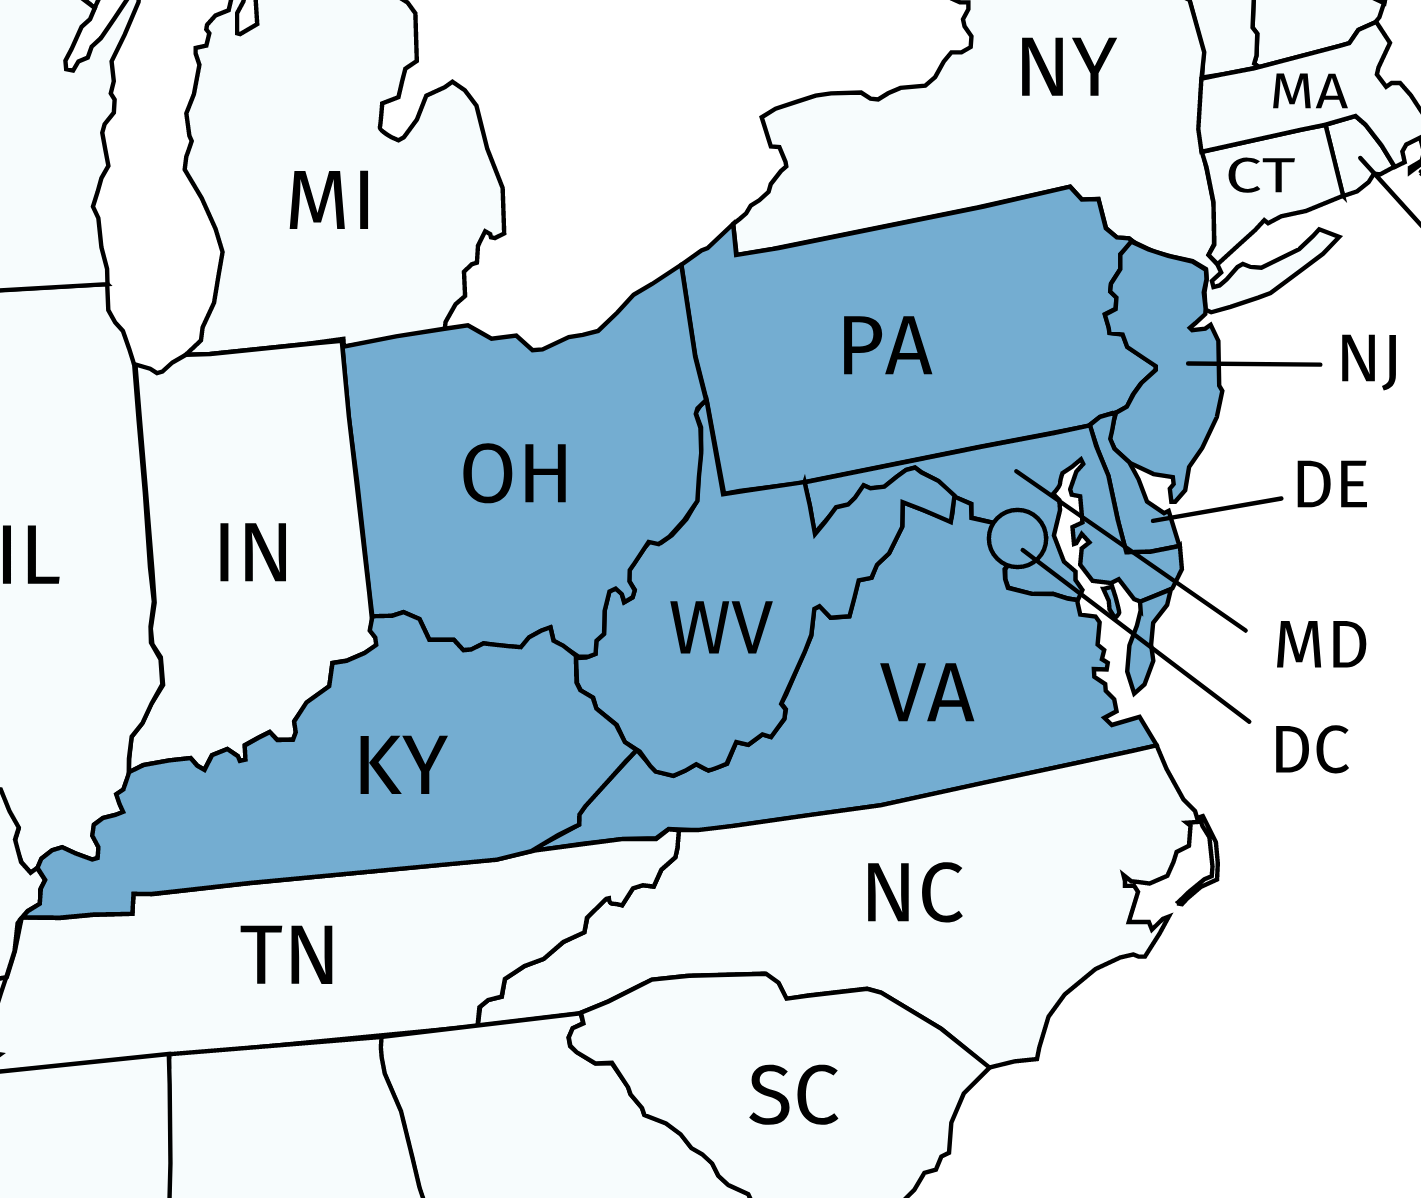
\includegraphics[height=2.8in]{selected_states_around_md_cropped}
\end{center}}
\ptwo{The map below shows eight countries in Asia highlighted in blue.  Draw a graph to represent this map, where each node represents a country, and an edge represents a shared border between two countries.
\begin{center}
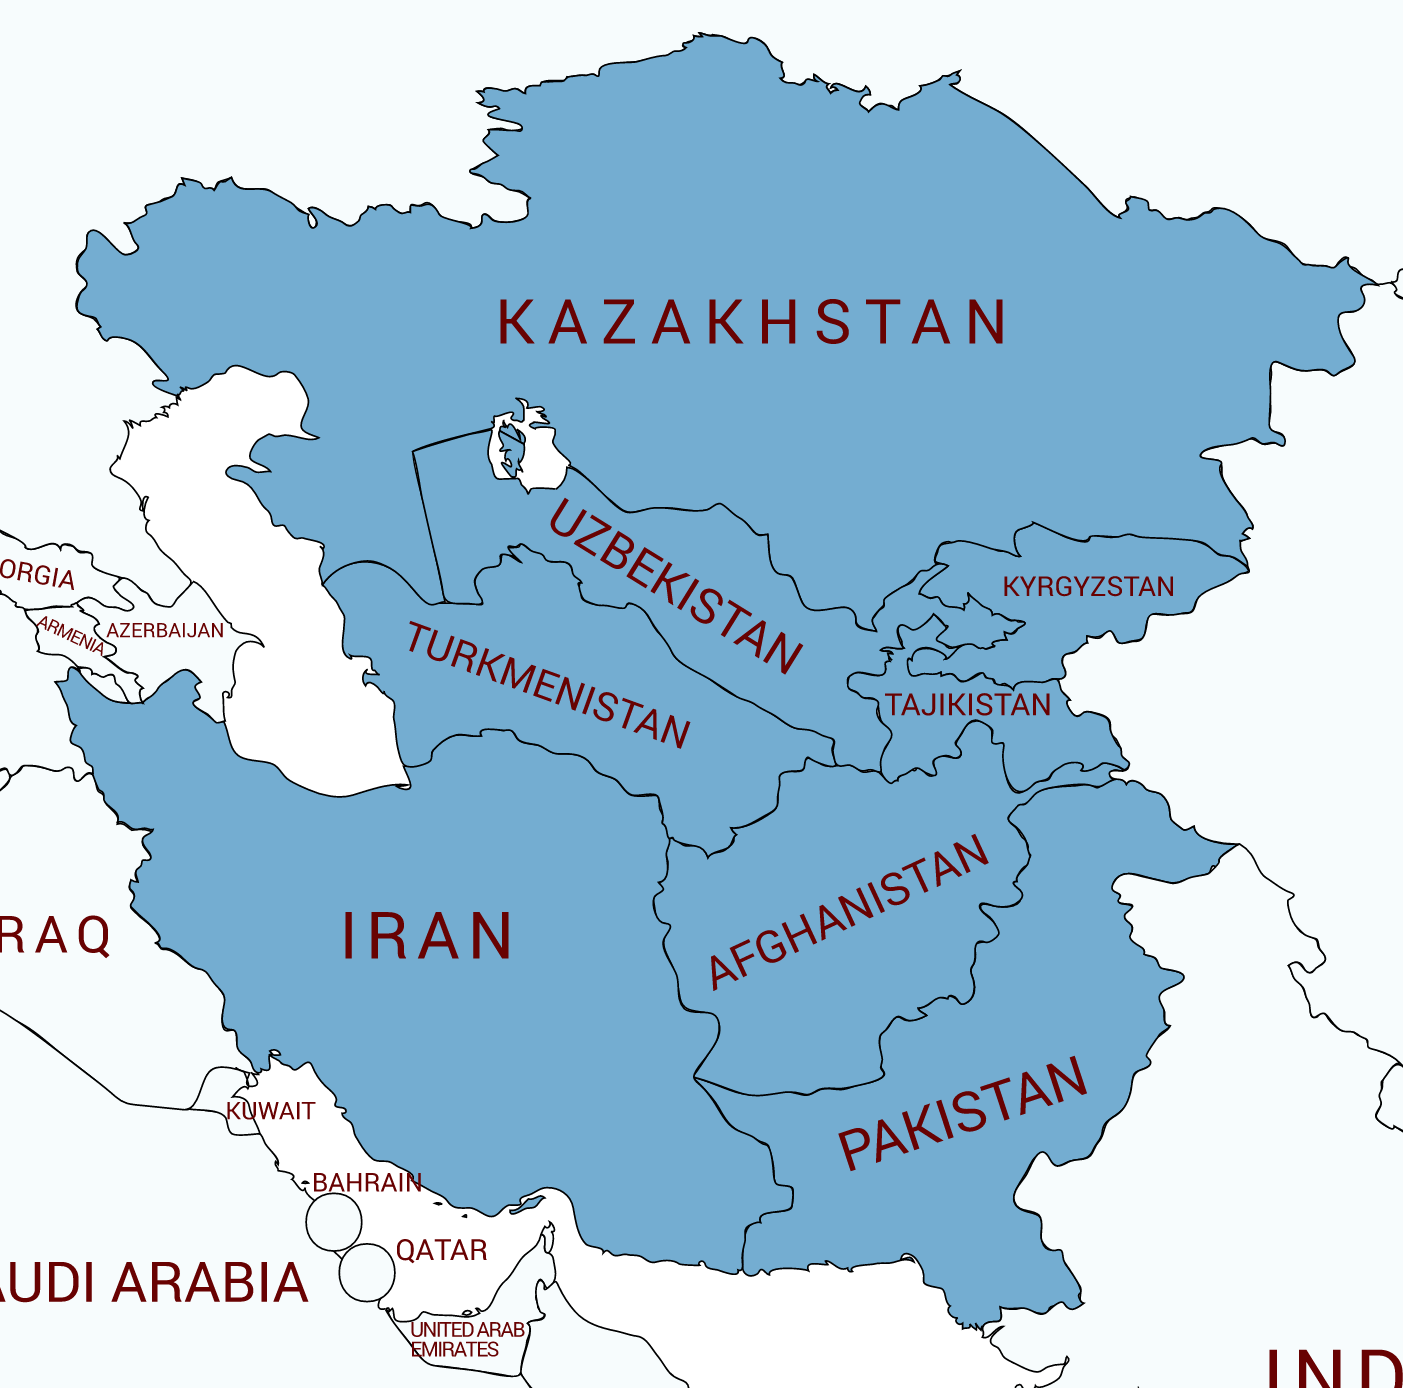
\includegraphics[height=2.8in]{middle_east_countries_cropped}
\end{center}}

\ptwo{The graph below represents a tournament; each edge marks a game between two teams.
\begin{center}
\begin{tikzpicture}
  \GraphInit[vstyle=simple]
  \tikzset{VertexStyle/.append style={scale=0.3}}
  \SetGraphUnit{1}
  
  \grEmptyCycle[RA=1.5,rotation=18,prefix=a]{5}
  
  \extralabel[1mm]{a0}{0}{Warriors}
  \extralabel[1mm]{a1}{90}{Hawks}
  \extralabel[1mm]{a2}{180}{Hornets}
  \extralabel[1mm]{a3}{-90}{Lions}
  \extralabel[1mm]{a4}{-90}{Bears}
  
  \Edge(a1)(a0)
  \Edge(a1)(a3)
  \Edge(a2)(a4)
  \Edge(a2)(a0)
  \Edge(a4)(a0)
  \Edge(a2)(a3)
  \Edge(a0)(a3)
\end{tikzpicture}
\end{center}
\begin{enumerate}[(a)]
\item Did the Hornets and the Hawks play each other?
\item How many games do the Warriors play?
\item Which teams do the Bears play?
\item Which team(s) played the most games?
\item Which team(s) played the fewest games?
\end{enumerate}}
\ptwo{The graph below is an \emph{influence graph}, where each edge represents the influence that one person has on another; the arrow goes from the influencer to the one they influence.
\begin{center}
\begin{tikzpicture}
  \GraphInit[vstyle=simple]
  \tikzset{VertexStyle/.append style={scale=0.3}}
  \SetGraphUnit{1.8}
  
  \Vertex{Joelle}
  \EA(Joelle){Jonathan}
  \SO(Joelle){Anastasia}
  \SO(Jonathan){Laila}
  \EA(Laila){Zachary}
  
  \extralabel[1mm]{Joelle}{90}{Joelle}
  \extralabel[1mm]{Jonathan}{90}{Jonathan}
  \extralabel[1mm]{Anastasia}{-90}{Anastasia}
  \extralabel[1mm]{Laila}{-90}{Laila}
  \extralabel[1mm]{Zachary}{0}{Zachary}
  
  \tikzset{EdgeStyle/.style = {->-,>=latex[round]}}
  \Edge(Zachary)(Jonathan)
  \Edge(Zachary)(Laila)
  \Edge(Zachary)(Joelle)
  \Edge(Anastasia)(Jonathan)
  \Edge(Joelle)(Laila)
  \Edge(Laila)(Jonathan)
  \Edge(Anastasia)(Joelle)
\end{tikzpicture}
\end{center}
\begin{enumerate}[(a)]
\item Who does Laila influence?
\item Does Jonathan influence Anastasia?
\item How many people does Joelle influence?
\item Who is the most influential (influences the most people)?
\item Who is the most influenced (influenced by the most people)?
\end{enumerate}}
\pagebreak

\emph{For problems 7--10, describe a graph that could be used to model the given application.  Specifically, answer the following questions:
\begin{enumerate}[(a)]
\item Are loops allowed in this graph?
\item Are multiple edges allowed between the same pair of nodes?
\item Is this a simple graph or multigraph?
\item Is this graph directed or undirected?
\item Is this a complete graph (generally)?
\end{enumerate}}
\ptwo{Flights between major cities, if each node represents a city and each edge describes a flight from one city to another (or from a city to itself, if there is a sightseeing or training flight).}
\ptwo{A party, where each node represents a person, and each edge represents whether one person knows the name of another.}

\ptwo{The floorplan of a house, where each node represents a room or space (like a hallway), and each edge represents a doorway.}
\ptwo{Courses offered at a college, where each node represents a course, and each edge represents a prerequisite requirement.}

\emph{For problems 11--14, answer the following questions for the given graph:
\begin{enumerate}[(a)]
\item Is it a simple graph or multigraph?
\item Is it directed or undirected?
\end{enumerate}}
\pfour{\begin{center}
\begin{tikzpicture}
  \GraphInit[vstyle=simple]
  \tikzset{VertexStyle/.append style={scale=0.3}}
  \SetGraphUnit{2.2}
  
  \Vertex{a}
  \EA(a){b}
  \SO(a){c}
  \SO(b){d}
  
  \extralabel[1mm]{a}{90}{$a$}
  \extralabel[1mm]{b}{90}{$b$}
  \extralabel[1mm]{c}{-90}{$c$}
  \extralabel[1mm]{d}{-90}{$d$}
  
  %\tikzset{EdgeStyle/.style = {->-,>=latex[round]}}
  %\SetUpEdge[style={bend right=30}]
  %\Loop[dist=1.5cm,dir=NO,style={-}](NYC)
  \Edge(a)(b)
  \Edge(b)(d)
  \Edge(b)(c)
  \SetUpEdge[style={bend right=30}]
  \Edge(a)(d)
  \Edge(d)(a)
\end{tikzpicture}
\end{center}}
\pfour{\begin{center}
\begin{tikzpicture}
  \GraphInit[vstyle=simple]
  \tikzset{VertexStyle/.append style={scale=0.3}}
  \SetGraphUnit{2.2}
  
  \Vertex{a}
  \EA(a){b}
  \SO(a){c}
  \SO(b){d}
  
  \extralabel[1mm]{a}{90}{$a$}
  \extralabel[1mm]{b}{90}{$b$}
  \extralabel[1mm]{c}{-90}{$c$}
  \extralabel[1mm]{d}{-90}{$d$}
  
  \tikzset{EdgeStyle/.style = {->-,>=latex[round]}}
  %\SetUpEdge[style={bend right=30}]
  %\Loop[dist=1.5cm,dir=NO,style={-}](NYC)
  \Edge(a)(c)
  \Edge(b)(c)
  \Edge(d)(b)
  \tikzset{EdgeStyle/.style = {->-,>=latex[round],bend right=30}}
  \Edge(a)(b)
  \Edge(b)(a)
\end{tikzpicture}
\end{center}}
\pfour{\begin{center}
\begin{tikzpicture}
  \GraphInit[vstyle=simple]
  \tikzset{VertexStyle/.append style={scale=0.3}}
  \SetGraphUnit{0.75}
  
  \Vertex{a}
  \EA(a){b}
  \SOEA(b){c}
  \SOWE(c){d}
  \WE(d){e}
  \NOWE(e){f}
  
  \extralabel[1mm]{a}{90}{$a$}
  \extralabel[1mm]{b}{0}{$b$}
  \extralabel[1mm]{c}{0}{$c$}
  \extralabel[1mm]{d}{-90}{$d$}
  \extralabel[1mm]{e}{-90}{$e$}
  \extralabel[1mm]{f}{180}{$f$}
  
  %\tikzset{EdgeStyle/.style = {->-,>=latex[round]}}
  %\SetUpEdge[style={bend right=30}]
  \Loop[dist=1.2cm,dir=NO,style={-}](b)
  \Loop[dist=1.2cm,dir=WE,style={-}](e)
  \Edge(a)(b)
  \Edge(a)(b)
  \Edge(b)(c)
  \SetUpEdge[style={bend right=15}]
  \Edge(a)(d)
  \Edge(d)(a)
  \Edge(a)(e)
  \Edge(e)(f)
  \Edge(a)(d)
  \Edge(c)(f)
\end{tikzpicture}
\end{center}}
\pfour{\begin{center}
\begin{tikzpicture}
  \GraphInit[vstyle=simple]
  \tikzset{VertexStyle/.append style={scale=0.3}}
  \SetGraphUnit{1.8}
  
  \Vertex{a}
  \EA(a){b}
  \SO(a){c}
  \SO(b){d}
  \EA(b){e}
  
  \extralabel[1mm]{a}{90}{$a$}
  \extralabel[1mm]{b}{90}{$b$}
  \extralabel[1mm]{c}{-90}{$c$}
  \extralabel[1mm]{d}{-90}{$d$}
  \extralabel[1mm]{e}{0}{$e$}
  
  \tikzset{EdgeStyle/.style = {->-,>=latex[round]}}
  \Edge(a)(b)
  \Edge(c)(a)
  \Edge(a)(d)
  \Edge(b)(e)
  \Edge(e)(d)
  \Edge(d)(b)
\end{tikzpicture}
\end{center}}

\emph{For problems 15--17, determine the degree of each node.  For the directed graphs, determine both the in-degree and the out-degree of each node.}\\
\pthree{\begin{center}
\begin{tikzpicture}
  \GraphInit[vstyle=simple]
  \tikzset{VertexStyle/.append style={scale=0.3}}
  \SetGraphUnit{2}
  
  \Vertex{a}
  \EA(a){b}
  \SO(a){c}
  \SO(b){d}
  \EA(b){e}
  
  \extralabel[1mm]{a}{90}{$a$}
  \extralabel[1mm]{b}{90}{$b$}
  \extralabel[1mm]{c}{-90}{$c$}
  \extralabel[1mm]{d}{-90}{$d$}
  \extralabel[1mm]{e}{0}{$e$}
  
  \tikzset{EdgeStyle/.style = {->-,>=latex[round]}}
  \Loop[dist=1.2cm,dir=NO,style={->-}](b)
  \Edge(b)(c)
  \Edge(d)(e)
  \Edge(d)(b)
  \tikzset{EdgeStyle/.style = {->-,>=latex[round],bend right=15}}
  \Edge(a)(c)
  \Edge(c)(a)
  \Edge(b)(e)
  \Edge(e)(b)
\end{tikzpicture}
\end{center}}
\pthree{\begin{center}
\begin{tikzpicture}
  \GraphInit[vstyle=simple]
  \tikzset{VertexStyle/.append style={scale=0.3}}
  
  \grEmptyCycle[RA=1.7,prefix=a]{6}
  
  \extralabel[1mm]{a0}{0}{$a$}
  \extralabel[1mm]{a1}{90}{$b$}
  \extralabel[1mm]{a2}{90}{$c$}
  \extralabel[1mm]{a3}{180}{$d$}
  \extralabel[1mm]{a4}{-90}{$e$}
  \extralabel[1mm]{a5}{-90}{$f$}
  
  %\tikzset{EdgeStyle/.style = {->-,>=latex[round]}}
  %\SetUpEdge[style={bend right=30}]
  %\Loop[dist=1.5cm,dir=NO,style={-}](NYC)
  \Edge(a0)(a1)
  \Edge(a0)(a3)
  \Edge(a1)(a4)
  \Edge(a2)(a4)
  \Edge(a3)(a5)
  \SetUpEdge[style={bend right=20}]
  \Edge(a1)(a5)
  \Edge(a5)(a1)
\end{tikzpicture}
\end{center}}
\pthree{\begin{center}
\begin{tikzpicture}
  \GraphInit[vstyle=simple]
  \tikzset{VertexStyle/.append style={scale=0.3}}
  \grComplete[RA=1.7,prefix=a]{7}
  
  \extralabel[1mm]{a0}{0}{$a$}
  \extralabel[1mm]{a1}{45}{$b$}
  \extralabel[1mm]{a2}{90}{$c$}
  \extralabel[1mm]{a3}{135}{$d$}
  \extralabel[1mm]{a4}{180}{$e$}
  \extralabel[1mm]{a5}{-90}{$f$}
  \extralabel[1mm]{a6}{-45}{$g$}
\end{tikzpicture}
\end{center}}

\end{exercises}